\definecolor{verde_p}{rgb}{0.67,0.87,0.74}

\chapter{Desarrollo del proyecto}

\section{Planteamiento inicial}

El desarrollo se ha llevado a cabo de manera modular. Se ha planteado el trabajo en bloques individuales para terminar comunicándolos por su respectiva vía.

Los objetivos descritos en la sección \ref{sec:refobj} sirven de guía para definir responsabilidades de cada módulo.

En la figura \ref{fig:diainteraccion} se puede observar el diagrama de interacciones entre los diferentes módulos

\begin{figure}[tb]
\centering
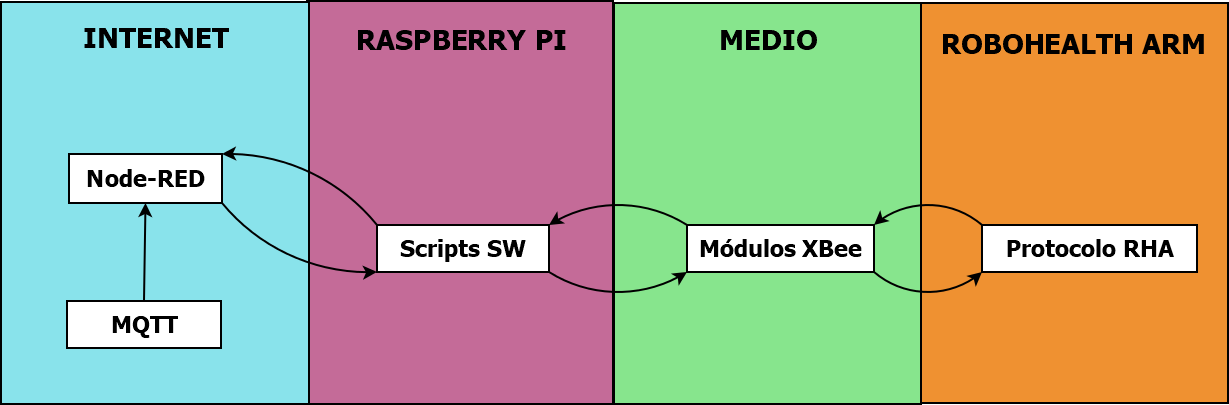
\includegraphics[width=1\textwidth]{figuras/DiaInteraccion.png}
\caption{Diagrama de interacción}
\label{fig:diainteraccion}
\end{figure}

Se establece una comunicación bidireccional en la que, por un lado, se envían comandos desde varias fuentes de mando y, por el otro, se reciben los mensajes periódicos de estado que envía el RoboHealth Arm.

Las fuentes de mando se emplazan en la red, desde donde se interactúa con el usuario. Una de ellas es Node-RED, la base de la red domótica y la otra es Mosquitto (MQTT), que diversifica el tipo de dispositivos desde los que se puede interactuar con el brazo.

La Raspberry Pi es el punto donde las órdenes enviadas desde la red toman forma en una salida serial.

Los módulos XBee se encargan de la transmisión inalámbrica de la información a través del medio\footnote{En la sección \ref{sec:radiofrec} se detalla el proceso del envío de ondas electromagnéticas a través del aire}.

Esta información es captada por el brazo robótico de acuerdo a un protocolo de comunicación prediseñado y actúa en consecuencia.

Haciendo una analogía con los diagramas de casos de uso propios del Lenguaje de Modelado Unificado (UML) en el campo del desarrollo software, a continuación (figura \ref{fig:diacasos})se analizan las distintas acciones que puede efectuar el usuario y cómo debería reaccionar el sistema ante estas acciones. Nótese que se ha tomado al brazo robótico como un actor más dentro del sistema domótico.

\begin{figure}[tb]
\centering
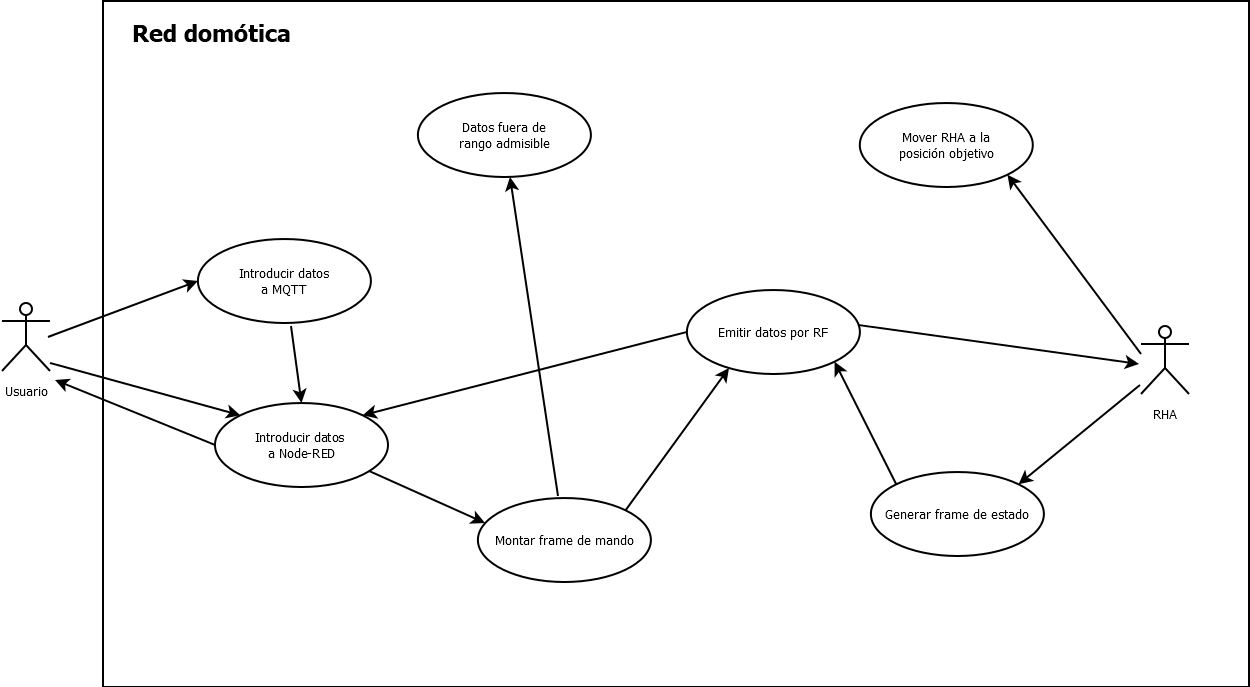
\includegraphics[width=1\textwidth]{figuras/DiaCasos.png}
\caption{Diagrama de casos de uso}
\label{fig:diacasos}
\end{figure}

Continuando con el uso de conceptos UML, en la imagen \ref{fig:diasecuencia} se puede observar la secuencia de acciones planificadas para el envío de información al brazo robótico.

\begin{figure}[tb]
\centering
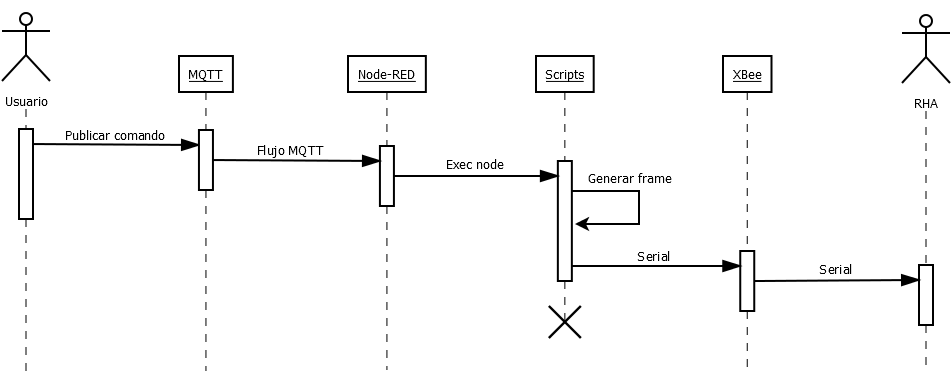
\includegraphics[width=1\textwidth]{figuras/DiaSecuencia.png}
\caption{Diagrama de Secuencia de envío}
\label{fig:diasecuencia}
\end{figure}

Con los objetivos y conceptos establecidos, se puede pasar al desarrollo siguiendo una metodología modular, como se ha indicado antes.

\section{Unidad de mando}

La base de las comunicaciones debe ser un ordenador. Las funciones de este ordenador o unidad de mando pasan por la coordinación de los diferentes elementos de la red domótica, incluyendo tanto el control de estos como la recepción de sus estados.

Es posible (y deseable) que ciertos elementos tengan otro control independiente a la red domótica. Así, por ejemplo, una persiana conectada a la red domótica podría ser accionada por el mismo ordenador sin obviar que el mecanismo podría accionarse a través de un pulsador. Esto hace necesaria la monitorización de la mayor parte posible de elementos. Podría darse el caso de que, incluso, la acción de ciertos elementos fuera mecánica en complementación a la acción de naturaleza electrica, imposibilitando cualquier integración de estos métodos alternativos de accionamiento en la red domótica. 

La unidad de mando debe encargarse de igual manera de la interacción con el usuario, aportando una interfaz.

Los requisitos de un sistema domótico no son especialmente exigentes en cuanto a la capacidad de procesamiento, por lo que características como un tamaño contenido o un bajo coste se valoran positivamente en la elección del ordenador0
.
En este contexto, se hace uso de la popular Raspberry Pi 3 Model B (figura \ref{fig:RPi3}) para el cometido descrito.

\subsection{Rasberry Pi 3 Model B}

La Raspberry Pi 3 Model B es uno de los más actuales modelos\footnote{Sólo se encuentra la Raspberry Pi 3 Model B+ con una fecha de lanzamiento posterior} de la tercera generación de este popular micro-ordenador de bajo coste. Si se miran sus especificaciones, se puede observar que, corriendo a través de una CPU Broadcom BCM2837 de 64 bits a 1.2GHz, posee:

\begin{itemize}
\item 1GB de memoria RAM
\item Conexión LAN inalámbrica y módulo Bluetooth integrados
\item Puerto Ethernet
\item 40 pines de entrada/salida (GPIO)
\item 4 puertos USB 2.0
\item Salida stereo de 4 polos
\item Conector HDMI
\item Puerto de cámara CSI
\item Puerto de display DSI
\item Puerto microSD
\item Puerto microUSB
\end{itemize}

Se puede observar el layout de estos componentes sobre la placa en la figura \ref{fig:RPilayout}.

\begin{figure}[tb]
\centering
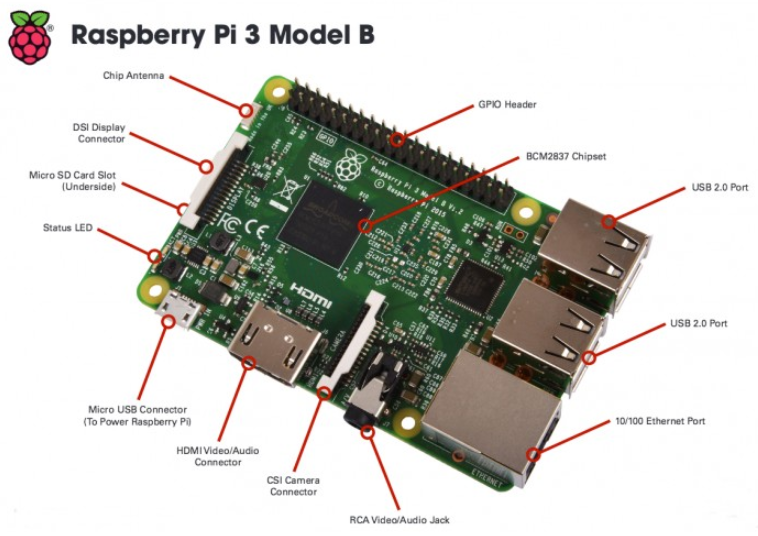
\includegraphics[width=0.5\textwidth]{figuras/RPiLayout.png}
\caption{Layout de puertos de la Raspberry Pi}
\label{fig:RPilayout}
\end{figure}

El puerto microUSB tiene la función de alimentar al ordenador. Se debe conectar una alimentación de 5 voltios a 2.5 amperios. Podría funcionar con una fuente de menos potencia pero podría ser que no soportara la inclusión de ciertos periféricos.

El puerto microSD sirve de alojamiento para la memoria ROM de la Raspberry. A través de este puerto, se carga el sistema operativo y se utiliza la memoria libre como almacenamiento interno.

\subsubsection{Raspbian OS}

Raspbian OS es el sistema operativo utilizado en la Raspberry Pi del laboratorio (figura \ref{fig:raspbian}. Se trata de una distribución no oficial basada en Debian adaptada a las especificaciones de la placa computadora Raspberry Pi. Debian está basado en el sistema GNU/Linux y, por tanto, se habla de software libre. El software, con sus características y actualizaciones, es desarrollado por la comunidad.

\begin{figure}[tb]
\centering
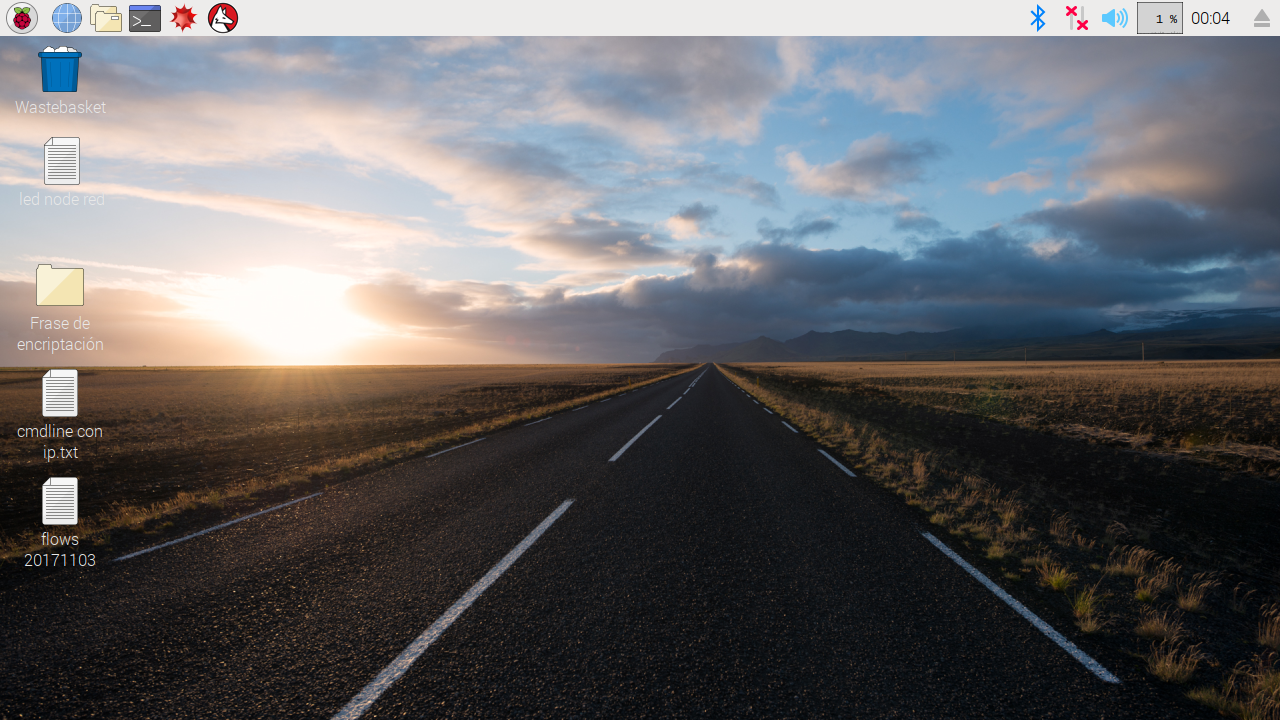
\includegraphics[width=0.5\textwidth]{figuras/Raspbian.png}
\caption{Escritorio de Raspbian}
\label{fig:raspbian}
\end{figure}

Entre otras funcionalidades, destaca el poder configurar la Raspberry de manera sencilla a través del menú \textit{raspy-config}

En el Anexo \ref{anexo:raspbian} se encuentran las instrucciones para obtener Raspbian 9.1 (Stretch) instalado en la Raspberry. Esta es la última distribución estable a día de hoy.

\subsubsection{Comunicación con otros ordenadores}

% Configuración de la visualización del código SW
\lstset{backgroundcolor=\color{verde_p}, language=bash, breaklines=true, basicstyle=\footnotesize, xleftmargin=25pt, framesep=8pt, numbersep=15pt}

A la hora de trabajar con la Raspberry instalada, no es usual que sea deseable la instalación de periféricos de entrada y salida para interactuar con ella. Es por esto por lo que se recurre a una conexión SSH para trabajar desde remoto con otro ordenador exactamente de igual manera a la que lo haríamos desde la ventana de comandos de Linux.

El procedimiento es diferente en función de si la conexión se efectúa desde una máquina en Linux o en Windows

\begin{itemize}
\item \textbf{Conexión SSH desde Windows}

En Windows existen varios programas dedicados a establecer conexiones entre dispositivos. Uno de los más conocidos es \textbf{Putty} (figura \ref{fig:putty}), en cuya interfaz puedes introducir la dirección IP del cliente\footnote{La dirección IP de la Raspberry Pi se puede obtener usando el comando \textit{ifconfig} una vez la conexión a internet ya ha sido establecida}, un puerto libre y el tipo de conexión que deseas (SSH, en nuestro caso). Al pulsar \textit{Open} se abre un terminal en el que se solicitan las credenciales antes de tener acceso completo a la Raspberry.

\begin{figure}[tb]
\centering
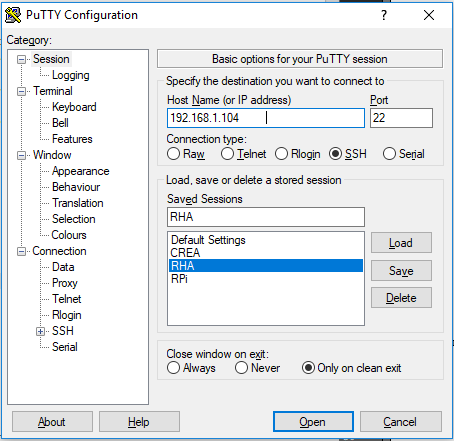
\includegraphics[width=0.5\textwidth]{figuras/Putty.png}
\caption{Interfaz de Putty}
\label{fig:putty}
\end{figure}

\item \textbf{Conexión SSH desde Linux}

En Linux se puede establecer una conexión SSH haciendo uso del terminal

\begin{lstlisting}[frame=single, label=command:ssh]
ssh root@190.168.1.104
\end{lstlisting}

El comando \textit{ssh} establece este tipo de conexiones. El usuario se indica en el lugar de \textit{root} en el ejemplo mientras que la IP del remoto se sitúa después del arroba. Es posible configurar el puerto con la opción \textit{-p} (por defecto se usa el puerto 22).

\begin{lstlisting}[frame=single, label=command:ssh]
ssh -p 22 root@190.168.1.104
\end{lstlisting}

De igual manera que en Windows, se solicitará la contraseña del usuario si procede y se accederá al terminal.

\end{itemize}

\subsection{MQTT}

Mosquitto (Message Queue Telemetry Transport) es un protocolo de código abierto enfocado a las conexiones Machine-to-Machine (M2M) \cite{Vega:2016} que se ha popularizado entre diferentes aplicaciones que precisan de comunicación entre sensores y mandos de redes domóticas. Entre sus características se encuentra un consumo de recursos muy bajo.

Su funcionamiento se basa en una configuración de estrella. Trabaja con un nodo central (también llamado Broker) con el que se establecen conexiones bidireccionales desde múltiples clientes (figura \ref{fig:mqtt}). Estas conexiones son cifradas, aportando una capa de seguridad a la red domótica.

\begin{figure}[b]
\centering
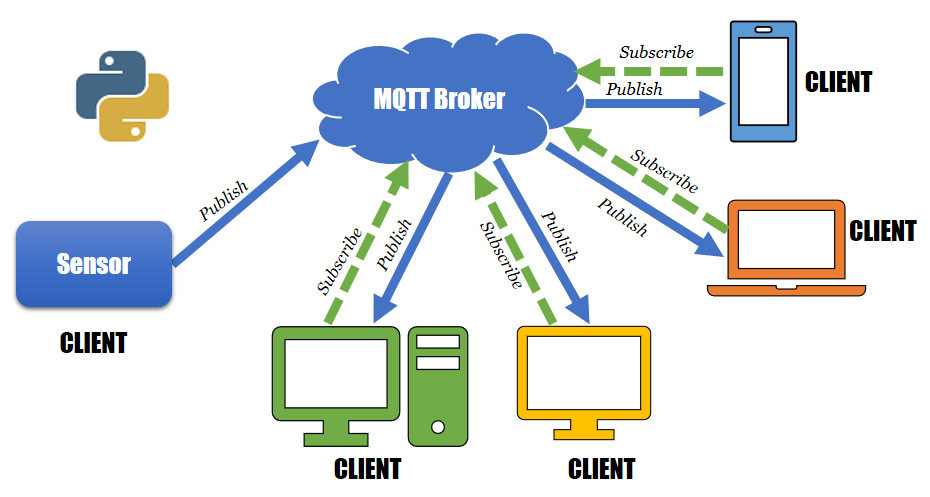
\includegraphics[width=0.5\textwidth]{figuras/mqtt.png}
\caption{Arquitectura MQTT}
\label{fig:mqtt}
\end{figure}

El concepto de \textit{topic} es la forma que tiene MQTT de articular las comunicaciones. Se puede hacer una analogía de los \textit{topic} con un tablón de anuncios. La gente puede publicar en el tablón lo que le plazca y esto será visto por aquellos que se paren a mirar el tablón. De igual manera funciona MQTT, cualquier cliente puede publicar en un \textit{topic} y este mensaje será recibido por aquellos clientes que estén suscritos a ese mismo \textit{topic}. Los \textit{topics}, además, son jerarquizables. Esto es, pueden generarse subtopics de manera recurrente con el fin de poder enviar mensajes únicamente a un grupo de clientes si se observa la red desde una perspectiva más global.

Existen varios \textit{Broker} de MQTT pero, con diferencia, el más popular es el llamado Mosquitto.

Una guía para su instalación puede encontrarse en el Anexo \ref{anexo:mqtt}

\subsubsection{MQTT en RoboHealt}

En cuanto al funcionamiento dentro de la habitación, existe un topic denominado \textit{Robohealth/room/devices} donde publican los distintos dispositivos mientras Node-RED está suscrito.

Los mensajes en el topic de la habitación siguen un mismo formato:

{'id':xx,'atrib1':'yy','atrib2':'zz',(...)}

\textit{xx} remplaza el identificador del cliente, único para cada dispositivo. RoboHealth Arm ha sido identificado con el número \textbf{99}.

\textit{atrib1}, \textit{atrib2} y sucesivos son atributos a los que se les quiere dar un valor. En el caso de los dispositivos digitales el atributo suele ser único, siendo denominado \textit{status}. En el caso de RoboHealth Arm es posible trasladarle dos atributos correspondientes a las coordenadas articulares objetivo del robot. Los atributos son \textbf{shoulder} para el hombro y \textbf{elbow} para el codo.

\textit{yy}, \textit{zz} y sucesivos son los valores correspondientes a los atributos. En el caso del brazo deberán pasarse las dos \textbf{coordenadas articulares en formato hexadecimal}.

\subsection{Node-RED}



\subsection{Python scripts}


\section{Transmisión de la información}

\subsection{XBee Shield}

\subsection{Módulos XBee}

\subsubsection{Modos de comunicación}

\subsubsection{XCTU}

\subsubsection{Perfiles de comunicación}


\section{RoboHealth Arm}

\subsection{Protocolo de comunicación RHA}

\subsection{Modificaciones a RHA}

\subsubsection{Modificaciones Hardware}

\subsubsection{Modificaciones Software}

\section{Integración}

\subsection{MQTT - Node-RED}

\subsubsection{Flujos MQTT}

\subsection{User Interface - Node-RED}

\subsubsection{Flujos UI/Node-RED}

\subsection{Node-Red - XBee}

\subsection{XBee - RHA}
